\documentclass[12pt,a4paper]{article}

\usepackage[T1]{fontenc}
\usepackage[utf8]{inputenc}
\usepackage{lmodern}
\usepackage{microtype}
\usepackage{geometry}
\usepackage{booktabs}
\usepackage{longtable}
\usepackage{array}
\usepackage{tabularx}
\usepackage{enumitem}
\usepackage{xcolor}
\usepackage{url}
\usepackage{fancyhdr}
\usepackage{listings}
\usepackage{tikz}
\usepackage{pgfplots}
\usepackage{caption}

\usetikzlibrary{arrows.meta,positioning,shapes.geometric}
\pgfplotsset{compat=1.18}
\geometry{top=2.5cm,bottom=2.5cm,left=2.7cm,right=2.7cm}
\setlength{\parindent}{1.25cm}
\setlength{\parskip}{0.15cm}
\setlength{\headheight}{14pt}
\setlist{nosep,leftmargin=1.1cm}

\definecolor{azulporto}{HTML}{0B4F6C}
\definecolor{azulclaro}{HTML}{DCEEF5}
\definecolor{verdepass}{HTML}{287D3C}
\definecolor{vermelhofail}{HTML}{A11D33}
\definecolor{cinzafundo}{HTML}{F4F6F7}
\definecolor{cinzatexto}{HTML}{40484C}

\pagestyle{fancy}
\fancyhf{}
\fancyhead[L]{\small Portos Conectados}
\fancyhead[R]{\small Prova de conceito}
\fancyfoot[C]{\thepage}
\renewcommand{\headrulewidth}{0.3pt}

\lstdefinestyle{terminal}{
  basicstyle=\ttfamily\small,
  backgroundcolor=\color{cinzafundo},
  frame=single,
  rulecolor=\color{azulclaro},
  breaklines=true,
  columns=fullflexible,
  keepspaces=true,
  showstringspaces=false,
  aboveskip=0.7em,
  belowskip=0.7em
}
\lstset{style=terminal}

\newcommand{\pass}{\textcolor{verdepass}{\textbf{PASS}}}
\newcommand{\skipresult}{\textcolor{cinzatexto}{\textbf{SKIPPED}}}
\newcommand{\nottested}{\textcolor{vermelhofail}{\textbf{NÃO TESTADO}}}
\newcommand{\code}[1]{\texttt{#1}}
\renewcommand{\contentsname}{Sumário}
\renewcommand{\abstractname}{Resumo}
\renewcommand{\figurename}{Figura}
\renewcommand{\tablename}{Tabela}
\renewcommand{\refname}{Referências}

\begin{document}

\begin{titlepage}
  \centering
  \vspace*{1.6cm}
  {\color{azulporto}\rule{\textwidth}{2pt}}\\[1.2cm]
  {\Huge\bfseries Portos Conectados\\[0.35cm]}
  {\LARGE Prova de conceito de uma bancada de dados e comunicação}\par
  \vspace{0.7cm}
  {\Large MQTT real, consumer Python e InfluxDB real}\par
  \vspace{1.2cm}
  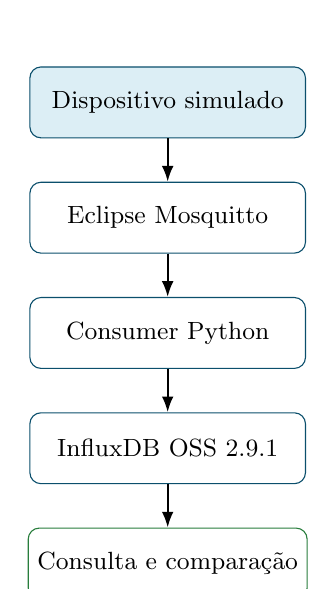
\begin{tikzpicture}[node distance=0.55cm, every node/.style={font=\small}]
    \node[draw=azulporto,rounded corners,fill=azulclaro,minimum width=3.5cm,minimum height=0.9cm] (sim) {Dispositivo simulado};
    \node[draw=azulporto,rounded corners,below=of sim,minimum width=3.5cm,minimum height=0.9cm] (mqtt) {Eclipse Mosquitto};
    \node[draw=azulporto,rounded corners,below=of mqtt,minimum width=3.5cm,minimum height=0.9cm] (consumer) {Consumer Python};
    \node[draw=azulporto,rounded corners,below=of consumer,minimum width=3.5cm,minimum height=0.9cm] (influx) {InfluxDB OSS 2.9.1};
    \node[draw=verdepass,rounded corners,below=of influx,minimum width=3.5cm,minimum height=0.9cm] (query) {Consulta e comparação};
    \draw[-{Latex[length=2mm]},thick] (sim)--(mqtt);
    \draw[-{Latex[length=2mm]},thick] (mqtt)--(consumer);
    \draw[-{Latex[length=2mm]},thick] (consumer)--(influx);
    \draw[-{Latex[length=2mm]},thick] (influx)--(query);
  \end{tikzpicture}
  \vfill
  {\large Relatório técnico-acadêmico de prova de conceito}\par
  \vspace{0.3cm}
  {\large 8 de outubro de 2026}\par
  \vspace{0.8cm}
  {\color{azulporto}\rule{\textwidth}{2pt}}
\end{titlepage}

\pagenumbering{roman}

\begin{abstract}
Este relatório apresenta uma prova de conceito, executada integralmente em terminal, para a etapa de software posterior a um futuro Network Server LoRaWAN do projeto Portos Conectados. A bancada implementa um simulador de sondas com continuidade temporal, transporte por MQTT em um broker Eclipse Mosquitto real, consumo e validação em Python, persistência em InfluxDB real e verificação posterior por consulta e comparação dos valores. O critério de aprovação exige que cada mensagem seja publicada, recebida, validada, gravada, localizada por seu identificador e comparada com a leitura original.

No ambiente avaliado, a suíte automatizada obteve 20 testes aprovados e 2 ignorados de forma explícita. O fluxo completo confirmou 100 de 100 mensagens, sem perda, a 20,259 mensagens por segundo; uma execução adicional confirmou 1.000 de 1.000 mensagens, a 17,983 mensagens por segundo. A latência aumentou com a formação de fila: o percentil 95 passou de 2.217,452 ms no teste de 100 mensagens para 28.989,733 ms no teste de 1.000 mensagens. A escrita direta em lote no InfluxDB confirmou 1.000 pontos em todas as configurações testadas e alcançou 22.669,311 pontos por segundo com lote 1.000. Também foram validadas deduplicação, detecção de ordem, fila SQLite durante indisponibilidade do banco, reconexão MQTT e reinício do consumer.

Os resultados caracterizam esta máquina e esta configuração. RSSI, SNR e distância são simulados. Não foi executado ensaio de alcance físico LoRaWAN nem uma topologia em três computadores; portanto, nenhuma conclusão de alcance de rádio é apresentada.
\end{abstract}

\noindent\textbf{Palavras-chave:} Internet das Coisas; qualidade da água; MQTT; InfluxDB; séries temporais; LoRaWAN; teste de software.

\newpage
\tableofcontents
\newpage
\pagenumbering{arabic}

\section{Introdução}

O projeto Portos Conectados pretende monitorar temperatura, pH, turbidez, condutividade e oxigênio dissolvido por sondas que futuramente usarão LoRaWAN. Antes da disponibilidade do rádio, do gateway e do Network Server, é possível investigar experimentalmente a infraestrutura que receberá os uplinks da aplicação. Esta prova de conceito, ou POC, foi construída como uma bancada reprodutível para esse propósito.

A arquitetura futura é composta por sensores, microcontrolador LoRaWAN, enlace de rádio, gateway, Network Server, MQTT, aplicação Python e InfluxDB. A POC substitui somente a parte anterior ao MQTT por um dispositivo simulado. O broker, a comunicação TCP/IP, o consumer, a escrita e a consulta ao banco são operações reais.

O princípio metodológico central é que aceitar uma requisição de escrita não prova a persistência. Uma execução é aprovada somente quando o mesmo \code{message\_id} é encontrado posteriormente no InfluxDB e os valores recuperados são iguais aos valores publicados.

\subsection{Objetivos}

O objetivo geral é implementar e avaliar uma bancada terminal para estudar o fluxo de dados MQTT--Python--InfluxDB antes da implantação do hardware LoRaWAN. Os objetivos específicos são:

\begin{itemize}
  \item formalizar o contrato mínimo das mensagens ambientais;
  \item medir entrega, latência, vazão, perda, duplicidade e ordem;
  \item comparar diferentes tamanhos de lote de escrita;
  \item observar o comportamento com mais dispositivos e mensagens;
  \item manter dados em fila local quando o InfluxDB estiver indisponível;
  \item verificar reconexão quando o MQTT cair;
  \item produzir evidências JSON, relatórios TXT/CSV e rastreamento individual;
  \item preparar a troca do simulador por um Network Server real sem reescrever o núcleo do consumer.
\end{itemize}

\subsection{Perguntas experimentais}

Os ensaios foram organizados para responder se o banco recebeu os dados, se eles foram recuperados sem alteração, qual latência e vazão foram observadas, se houve perda ou duplicidade, como o sistema reagiu ao aumento de carga e o que ocorreu nas indisponibilidades. Questões que exigem rádio, gateway ou máquinas fisicamente distintas são mantidas como trabalho futuro.

\section{Escopo e terminologia experimental}

Três experimentos são conceitualmente separados:

\begin{table}[htbp]
\centering
\caption{Separação dos experimentos.}
\begin{tabularx}{\textwidth}{>{\bfseries}p{3cm} X X}
\toprule
Experimento & O que comprova & Situação nesta rodada \\
\midrule
Software local & MQTT, processamento, validação, armazenamento, consulta, latência e perdas no ambiente local & Executado \\
Rede entre computadores & Tráfego TCP/IP real entre hosts distintos & Não executado; houve apenas TCP/IP local \\
Campo LoRaWAN & Rádio, gateway, PDR, RSSI, SNR e alcance nas condições medidas & Não executado \\
\bottomrule
\end{tabularx}
\end{table}

No documento, \emph{medido} identifica uma observação obtida por relógios e contadores do sistema; \emph{calculado} identifica estatísticas derivadas, como média e percentis; \emph{simulado} identifica condições produzidas pelo software; e \emph{não testado} identifica ausência de evidência experimental.

Toda execução do simulador declara:

\begin{lstlisting}
RADIO MODE: SIMULATED
PHYSICAL RANGE VALIDATION: NOT PERFORMED
\end{lstlisting}

Valores sintéticos de \code{distance\_m}, RSSI, SNR ou perda exercitam o tratamento de metadados. Eles não demonstram alcance de LoRaWAN.

\section{Arquitetura implementada}

\begin{figure}[htbp]
\centering
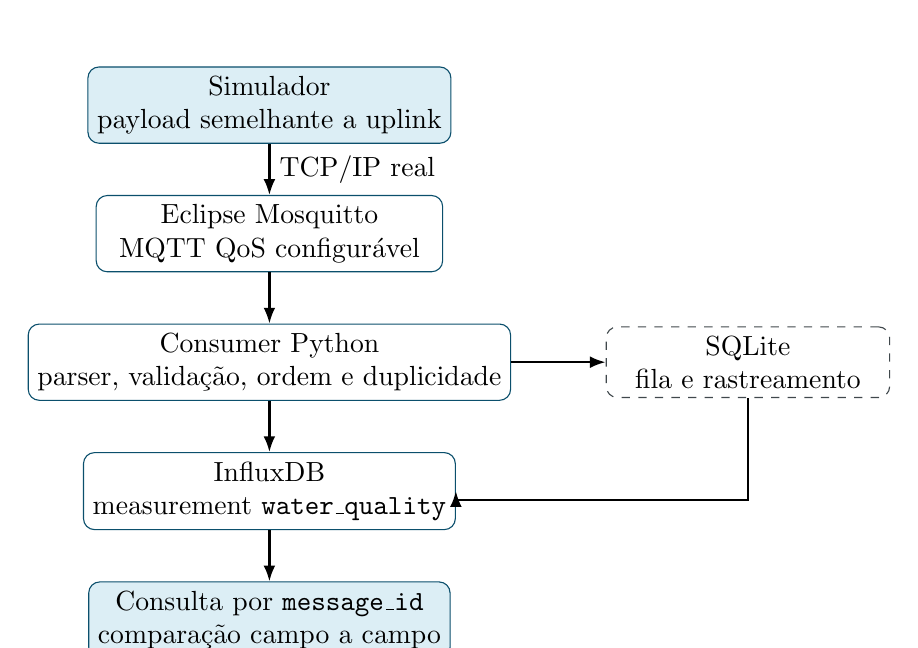
\begin{tikzpicture}[
  node distance=0.65cm,
  block/.style={draw=azulporto,rounded corners,minimum width=4.4cm,minimum height=0.85cm,align=center},
  side/.style={draw=cinzatexto,dashed,rounded corners,minimum width=3.6cm,minimum height=0.75cm,align=center},
  arrow/.style={-{Latex[length=2mm]},thick}
]
  \node[block,fill=azulclaro] (sim) {Simulador\\payload semelhante a uplink};
  \node[block,below=of sim] (broker) {Eclipse Mosquitto\\MQTT QoS configurável};
  \node[block,below=of broker] (parser) {Consumer Python\\parser, validação, ordem e duplicidade};
  \node[block,below=of parser] (influx) {InfluxDB\\measurement \code{water\_quality}};
  \node[block,fill=azulclaro,below=of influx] (query) {Consulta por \code{message\_id}\\comparação campo a campo};
  \node[side,right=1.2cm of parser] (sqlite) {SQLite\\fila e rastreamento};
  \draw[arrow] (sim)--node[right]{TCP/IP real}(broker);
  \draw[arrow] (broker)--(parser);
  \draw[arrow] (parser)--(influx);
  \draw[arrow] (influx)--(query);
  \draw[arrow] (parser)--(sqlite);
  \draw[arrow] (sqlite.south)--++(0,-1.3)-|(influx.east);
\end{tikzpicture}
\caption{Fluxo implementado na POC.}
\end{figure}

O payload simulado se aproxima do formato decodificado pelo The Things Stack. O parser está isolado em \code{consumer/parser.py}; assim, uma integração futura com The Things Stack ou ChirpStack deve adaptar o envelope externo e preservar o contrato interno.

\subsection{Componentes}

\begin{description}[style=nextline]
  \item[Simulador] Mantém um estado ambiental por dispositivo, aplica pequenas variações temporais e pode produzir uma alteração forte de turbidez. Cada dispositivo possui identificador e contador próprios.
  \item[MQTT] O Mosquitto recebe publicações no tópico configurado. O QoS é configurável e o padrão da bancada é 1.
  \item[Consumer] Recebe, converte o envelope, valida formato e valores, detecta repetição e ordem, escreve no banco e registra cada estágio.
  \item[Fila local] O SQLite preserva mensagens válidas quando o banco não responde. Uma pendência é removida apenas depois de escrita e consulta confirmadas.
  \item[InfluxDB] Armazena séries temporais e responde a consultas por \code{message\_id}. A implementação utilizada é compatível com a API 2.x e interrompe com mensagem clara se outra família for detectada.
  \item[CLI] Oferece menu, painel de estado, testes, rastreamento e explicações breves para apresentação.
\end{description}

\section{Contrato e qualidade dos dados}

\subsection{Campos}

\small
\begin{longtable}{>{\ttfamily\raggedright\arraybackslash}p{3.25cm} p{2.0cm} p{1.4cm} p{1.25cm} p{4.2cm}}
\caption{Contrato interno da leitura.}\\
\toprule
\normalfont Campo & Tipo & Unidade & Obrig. & Regra e armazenamento \\
\midrule
\endfirsthead
\toprule
\normalfont Campo & Tipo & Unidade & Obrig. & Regra e armazenamento \\
\midrule
\endhead
device\_id & texto & --- & sim & Não vazio; tag \\
message\_id & UUID & --- & sim & UUID válido; field e chave de deduplicação local \\
frame\_counter & inteiro & frame & rec. & Field; auxilia detecção de lacuna e ordem \\
gateway\_id & texto & --- & não & Tag \\
site & texto & --- & não & Tag de baixa cardinalidade \\
source & enum & --- & sim & \code{simulator} ou \code{lorawan-real}; tag \\
sent\_at & ISO 8601 & UTC & sim & Exige timezone; field \\
received\_at & ISO 8601 & UTC & sim no fluxo & Timestamp do ponto \\
temperature\_c & float & $^{\circ}$C & não & $-20$ a 80 aceito; fora rejeitado; field \\
ph & float & escala pH & não & 0 a 14; field \\
turbidity\_ntu & float & NTU & não & Negativo rejeitado; field \\
conductivity\_\allowbreak us\_cm & float & $\mu$S/cm & não & Negativo rejeitado; field \\
dissolved\_\allowbreak oxygen\_\allowbreak mg\_l & float & mg/L & não & Negativo rejeitado; field \\
rssi\_dbm & float & dBm & não & Field; simulado nesta rodada \\
snr\_db & float & dB & não & Field; simulado nesta rodada \\
distance\_m & float & m & não & Field; simulado nesta rodada \\
\bottomrule
\end{longtable}
\normalsize

Os limites são regras operacionais da POC e não critérios legais de qualidade da água. A validação separa formato inválido de valor ambiental suspeito. Por exemplo, \code{ph="abc"} é rejeitado; \code{ph=13.5} é numérico e aceito com alerta contextual. \code{NaN}, infinito, booleanos no lugar de números e turbidez negativa são rejeitados. Uma variável ambiental ausente permanece ausente e não é convertida em zero.

\subsection{Tempo, identidade e repetição}

Os timestamps usam ISO 8601 com timezone e são normalizados em UTC. \code{sent\_at} representa a geração no dispositivo; \code{received\_at}, o recebimento pelo envelope da infraestrutura. O timestamp do ponto é \code{received\_at}. A latência entre máquinas só pode ser interpretada se seus relógios estiverem sincronizados.

O UUID da mensagem é a identidade global utilizada no rastreamento. Como QoS 1 pode repetir uma entrega, o consumer mantém deduplicação local. Uma lacuna em \code{frame\_counter} indica possível ausência, mas não prova perda de rádio: reinício do dispositivo, rollover e retenção do broker também devem ser considerados no sistema definitivo.

\section{Modelo de dados no InfluxDB}

A instância detectada na execução foi InfluxDB OSS \textbf{v2.9.1}. A configuração exige URL, token, organização e bucket. O measurement é \code{water\_quality}.

As tags são \code{device\_id}, \code{gateway\_id}, \code{site} e \code{source}, pois são dimensões usadas para agrupar e filtrar. Variáveis numéricas, metadados de sinal, latência, distância e contador são fields. O UUID da mensagem também é field: transformá-lo em tag criaria uma série distinta para cada mensagem e elevaria a cardinalidade.

Um ponto do InfluxDB é identificado por measurement, conjunto de tags e timestamp. Escrever novamente essa identidade pode mesclar campos. A POC reduz ambiguidades com timestamps precisos e deduplicação pelo UUID antes da escrita. A retenção deve ser escolhida segundo prazo acadêmico, volume, necessidade histórica e política institucional; ela não é fixada como requisito científico universal.

O tamanho do lote, intervalo de flush, timeout e política de retry são parâmetros operacionais. A comparação experimental da Seção~\ref{sec:resultados} mostra que o lote altera fortemente a vazão, mas a seleção definitiva requer carga sustentada e recursos semelhantes aos da implantação.

\section{MQTT e preparação para LoRaWAN}

O contrato de comunicação inclui host, porta, tópico, QoS, autenticação, timeout e reconexão. Nenhum endereço é fixado no código: \code{MQTT\_HOST} e \code{INFLUX\_URL} podem apontar para outras máquinas. Credenciais ficam em \code{.env}, arquivo ignorado pelo Git.

No fluxo futuro, LoRa é a camada de rádio; LoRaWAN define acesso e gerenciamento da rede; a sonda é o End Device; o gateway encaminha quadros pela Internet; Network Server e Application Server processam e entregam o uplink; MQTT disponibiliza esse uplink à aplicação; e o InfluxDB preserva a série temporal. The Things Stack e ChirpStack diferem em tópicos, autenticação e envelopes. A fronteira do parser permite adaptar essas diferenças.

O hardware definitivo ainda exige dispositivo e gateway compatíveis com a região, conectividade, credenciais, DevEUI, JoinEUI/AppEUI quando aplicável, AppKey em OTAA, plano regional definido segundo a regulamentação aplicável, decoder, tópico, segurança, estratégia de retransmissão, intervalo de uplink, relógio e orçamento energético.

\section{Metodologia de teste}

\subsection{Ambiente}

\begin{table}[htbp]
\centering
\caption{Ambiente efetivamente utilizado.}
\begin{tabular}{ll}
\toprule
Elemento & Versão ou configuração \\
\midrule
Sistema operacional & Windows \\
Python & 3.14.6 \\
pytest & 9.1.1 \\
Eclipse Mosquitto & 2.1.2 \\
InfluxDB OSS & v2.9.1 \\
MQTT principal & \code{127.0.0.1:1883}, QoS 1 \\
Broker controlado de falha & \code{127.0.0.1:1884} \\
Measurement & \code{water\_quality} \\
\bottomrule
\end{tabular}
\end{table}

\subsection{Critério end-to-end}

Para cada mensagem, o teste:

\begin{enumerate}
  \item gera uma leitura com UUID único;
  \item publica o envelope no broker MQTT real;
  \item aguarda o subscriber do consumer;
  \item executa parser, validação e controle de duplicidade/ordem;
  \item grava a leitura no InfluxDB real;
  \item consulta o InfluxDB pelo UUID;
  \item compara campos originais e recuperados.
\end{enumerate}

Se uma das 100 mensagens esperadas não for encontrada, o teste de 100 termina como falha. A aprovação não é inferida da ausência de exceções.

\subsection{Métricas}

A vazão é o total confirmado dividido pelo tempo do ensaio. A perda é a diferença entre geradas e localizadas no banco. Os percentis P50, P95 e P99 são calculados sobre as latências observadas. No fluxo completo, a latência por mensagem corresponde ao intervalo entre geração e escrita registrada pelo consumer; a consulta posterior fornece a prova de existência. Os horários de todos os estágios são preservados no rastreamento.

\subsection{Falhas controladas}

Para o InfluxDB, o teste utiliza um destino indisponível, verifica a persistência no SQLite, restaura o writer correto, reprocessa a fila, consulta o UUID e só então remove a pendência. Para MQTT, uma instância real do Mosquitto é iniciada em porta isolada, encerrada e iniciada novamente. O consumer precisa detectar a queda, permanecer vivo, reconectar, receber nova mensagem e confirmá-la no banco.

\section{Resultados}\label{sec:resultados}

\subsection{Suíte automatizada}

A execução final de \code{python -m pytest -ra}, com \code{RUN\_INTEGRATION=1}, coletou 22 testes: \textbf{20 passaram}, \textbf{2 foram ignorados} e nenhum falhou, em 9,69 segundos. Os ignorados foram o teste de hardware LoRaWAN, por ausência de dispositivo e gateway, e a carga extensa, que exige ativação explícita para não sobrecarregar a máquina. Eles não foram contabilizados como aprovados.

\begin{table}[htbp]
\centering
\caption{Testes funcionais e de falha.}
\begin{tabularx}{\textwidth}{X c X}
\toprule
Teste & Resultado & Evidência principal \\
\midrule
MQTT isolado & \pass & UUID idêntico; 19,884 ms \\
InfluxDB isolado & \pass & 25,123456 $^{\circ}$C e pH 7,654321 sem diferença \\
End-to-end, 100 & \pass & 100 geradas e 100 consultadas \\
Duplicidade e ordem & \pass & 1 duplicata, 1 fora de ordem e 3 lacunas detectadas \\
Fila e recuperação do InfluxDB & \pass & pendência gravada, consultada e removida \\
Queda e retorno do MQTT & \pass & queda detectada, reconexão e confirmação no banco \\
Reinício do consumer & \pass & leituras antes/depois confirmadas; fila 0 \\
Evento ambiental simulado & \pass & 60/60 recebidas; 9 alterações sinalizadas \\
Hardware LoRaWAN & \skipresult & requisito físico ausente \\
\bottomrule
\end{tabularx}
\end{table}

\subsection{Fluxo completo}

\begin{table}[htbp]
\centering
\caption{Execuções end-to-end.}
\begin{tabular}{rrrrrrrr}
\toprule
Mens. & Sondas & Confirm. & Perda & msg/s & Média (ms) & P95 (ms) & P99 (ms) \\
\midrule
100 & 100 & 100 & 0 & 20,259 & 1.423,200 & 2.217,452 & 2.298,360 \\
1.000 & 10 & 1.000 & 0 & 17,983 & 17.566,275 & 28.989,733 & 29.555,505 \\
\bottomrule
\end{tabular}
\end{table}

Não houve perda nos dois ensaios. A latência, porém, cresceu de forma pronunciada na rajada maior. Isso evidencia formação de fila no caminho completo, que nesta versão escreve e registra individualmente cada mensagem. O teste de lote, apresentado adiante, isola o potencial do banco e mostra que o InfluxDB aceita vazão muito superior quando os pontos são agrupados.

\subsection{Escala por número de dispositivos}

Cada dispositivo publicou uma mensagem. Assim, este ensaio representa rajadas de tamanho crescente, e não carga sustentada por longos períodos.

\begin{table}[htbp]
\centering
\caption{Escala de uma mensagem por dispositivo.}
\begin{tabular}{rrrrrrr}
\toprule
Sondas & Mens. & Armaz. & Perda & msg/s & Média (ms) & P95 (ms) \\
\midrule
1 & 1 & 1 & 0 & 4,583 & 17,432 & 17,432 \\
10 & 10 & 10 & 0 & 16,542 & 172,858 & 244,340 \\
50 & 50 & 50 & 0 & 19,232 & 777,284 & 1.216,231 \\
100 & 100 & 100 & 0 & 19,803 & 1.319,238 & 2.121,202 \\
500 & 500 & 500 & 0 & 20,149 & 6.844,378 & 11.723,254 \\
\bottomrule
\end{tabular}
\end{table}

\begin{figure}[htbp]
\centering
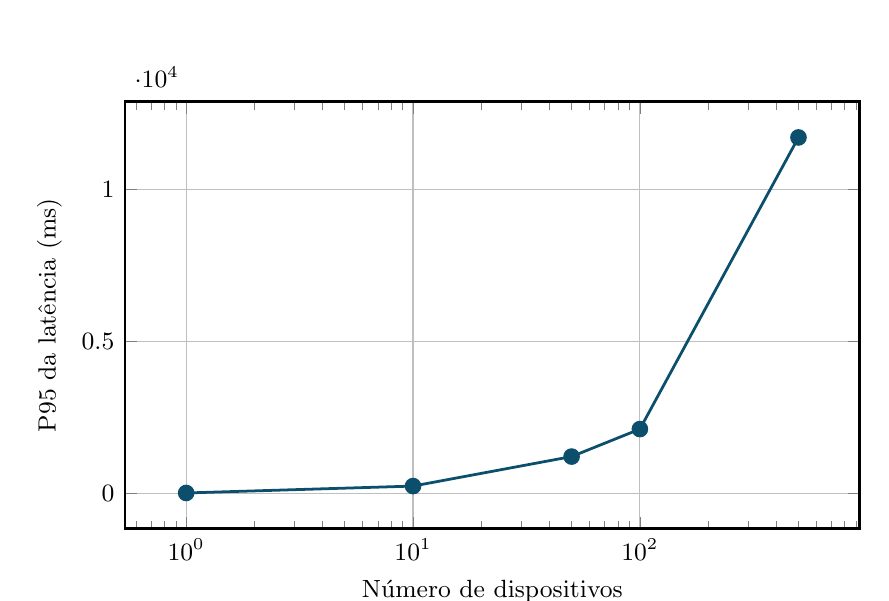
\begin{tikzpicture}
\begin{axis}[
  width=0.9\textwidth,height=7cm,
  xlabel={Número de dispositivos},ylabel={P95 da latência (ms)},
  xmode=log,log basis x=10,
  grid=major,
  tick label style={font=\small},label style={font=\small},
  line width=1pt,mark size=2.5pt
]
\addplot[color=azulporto,mark=*] coordinates {(1,17.432) (10,244.34035) (50,1216.23135) (100,2121.20185) (500,11723.25395)};
\end{axis}
\end{tikzpicture}
\caption{Crescimento do P95 nas rajadas com mais dispositivos. Dados medidos; percentil calculado.}
\end{figure}

A vazão se aproximou de 20 mensagens por segundo, enquanto o P95 aumentou até 11,723 s com 500 mensagens simultâneas. A conclusão sustentada pelos dados é que o pipeline preservou todas as mensagens dessa rajada, mas acumulou espera.

\subsection{Escrita em lote no InfluxDB}

O teste escreveu 1.000 pontos para cada tamanho de lote e consultou posteriormente os 1.000 identificadores. Não houve erro nem ausência.

\begin{table}[htbp]
\centering
\caption{Comparação de lotes no InfluxDB.}
\begin{tabular}{rrrrrr}
\toprule
Lote & Localizados & Erros & Tempo (s) & pontos/s & Média/chamada (ms) \\
\midrule
1 & 1.000 & 0 & 2,377 & 420,639 & 2,377 \\
10 & 1.000 & 0 & 0,169 & 5.917,583 & 1,689 \\
100 & 1.000 & 0 & 0,062 & 16.124,481 & 6,200 \\
500 & 1.000 & 0 & 0,046 & 21.903,694 & 22,825 \\
1.000 & 1.000 & 0 & 0,044 & 22.669,311 & 44,109 \\
\bottomrule
\end{tabular}
\end{table}

\begin{figure}[htbp]
\centering
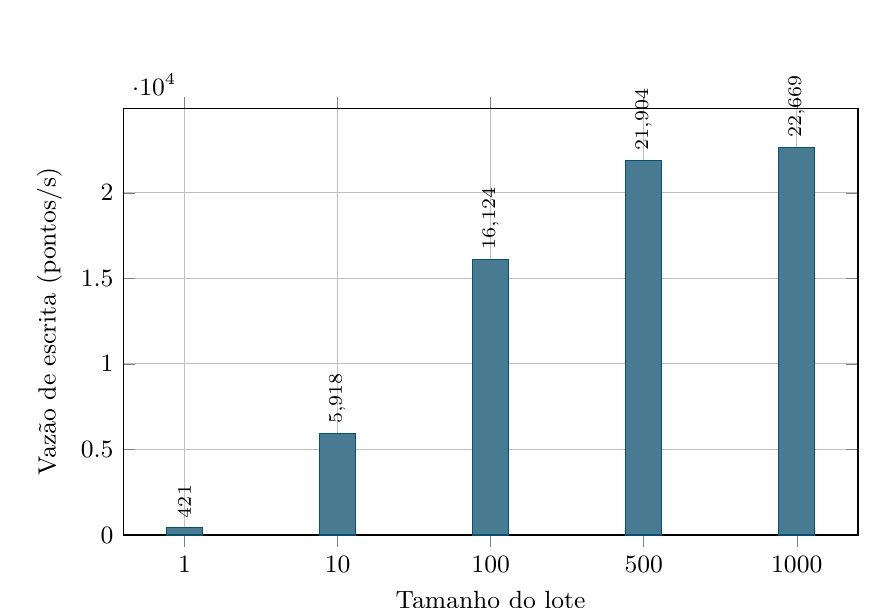
\begin{tikzpicture}
\begin{axis}[
  ybar,width=0.9\textwidth,height=7cm,
  xlabel={Tamanho do lote},ylabel={Vazão de escrita (pontos/s)},
  symbolic x coords={1,10,100,500,1000},xtick=data,
  ymin=0,grid=major,
  bar width=13pt,
  nodes near coords={\pgfmathprintnumber[fixed,precision=0]{\pgfplotspointmeta}},
  nodes near coords style={font=\scriptsize,rotate=90,anchor=west},
  tick label style={font=\small},label style={font=\small}
]
\addplot[fill=azulporto!75,draw=azulporto] coordinates {(1,420.639) (10,5917.583) (100,16124.481) (500,21903.694) (1000,22669.311)};
\end{axis}
\end{tikzpicture}
\caption{Vazão de escrita direta por tamanho de lote.}
\end{figure}

O lote 1.000 obteve a maior vazão agregada; o lote 10 apresentou a menor duração média por chamada. A escolha operacional depende do equilíbrio entre vazão, memória, tempo de espera para formar o lote e tolerância à perda de um lote em trânsito. A execução não autoriza generalização para outro hardware.

\subsection{Frequência solicitada e observada}

Foram publicadas amostras curtas de 20 mensagens em cada taxa. O limite de segurança era 1.000 mensagens por segundo e interrupção caso P95 ultrapassasse 10 s.

\begin{table}[htbp]
\centering
\caption{Teste indicativo de frequência.}
\begin{tabular}{rrrrrr}
\toprule
Solicitada & Observada & Armaz. & Perda & Média (ms) & P95 (ms) \\
\midrule
1 & 0,974 & 20 & 0 & 17,131 & 18,463 \\
10 & 8,274 & 20 & 0 & 16,537 & 17,372 \\
100 & 15,624 & 20 & 0 & 329,667 & 464,704 \\
500 & 18,686 & 20 & 0 & 312,171 & 443,791 \\
1.000 & 18,575 & 20 & 0 & 294,704 & 436,723 \\
\bottomrule
\end{tabular}
\end{table}

\begin{figure}[htbp]
\centering
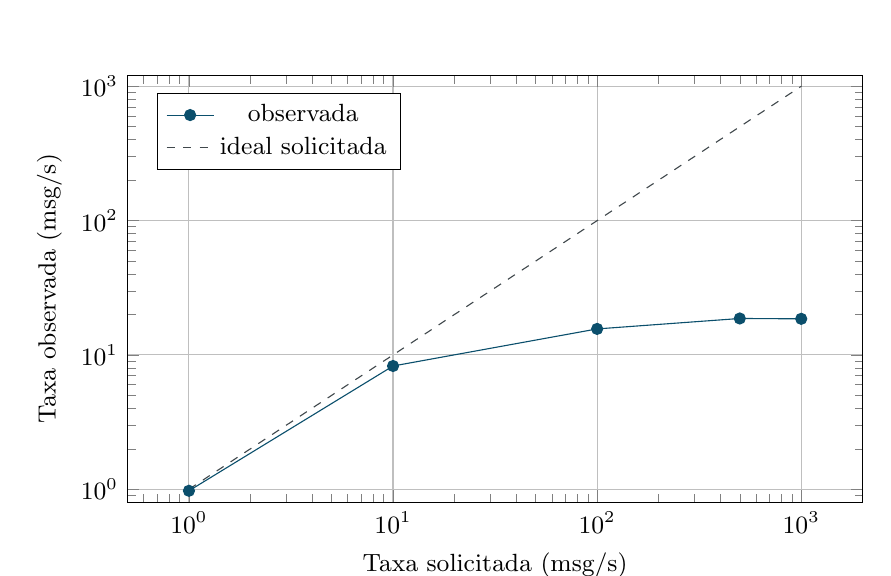
\begin{tikzpicture}
\begin{axis}[
  width=0.9\textwidth,height=7cm,
  xlabel={Taxa solicitada (msg/s)},ylabel={Taxa observada (msg/s)},
  xmode=log,log basis x=10,
  ymode=log,log basis y=10,ymin=0.8,ymax=1200,grid=major,
  legend style={at={(0.04,0.96)},anchor=north west,font=\small},
  tick label style={font=\small},label style={font=\small}
]
\addplot[color=azulporto,mark=*] coordinates {(1,0.9743) (10,8.2737) (100,15.6236) (500,18.6859) (1000,18.5752)};
\addlegendentry{observada}
\addplot[color=cinzatexto,dashed] coordinates {(1,1) (10,10) (100,100) (500,500) (1000,1000)};
\addlegendentry{ideal solicitada}
\end{axis}
\end{tikzpicture}
\caption{Taxa solicitada e vazão end-to-end observada em amostras curtas.}
\end{figure}

As amostras indicam saturação do pipeline individual perto de 19 mensagens por segundo nesse ambiente. Como cada ponto contém apenas 20 mensagens, o ensaio localiza a tendência, mas não determina uma taxa sustentável de produção. Essa determinação exige duração maior, monitoramento de CPU, memória e disco e repetição estatística.

\subsection{Falha e recuperação}

No teste de indisponibilidade do InfluxDB, uma mensagem válida foi enviada a um destino deliberadamente indisponível. Ela permaneceu no SQLite, foi reprocessada após a restauração, localizada por consulta e removida da fila. Resultado: \pass.

No teste MQTT, o broker 2.1.2 controlado na porta 1884 foi encerrado de fato. O consumer registrou a desconexão e permaneceu vivo. Depois da reinicialização, reconectou, recebeu o UUID \code{f9245534-b1da-4115-abec-20f4186f097f} e o confirmou no InfluxDB. Resultado: \pass.

No reinício do consumer, uma leitura anterior e outra posterior ao reinício foram confirmadas e a fila terminou em zero. Resultado: \pass.

\subsection{Evento ambiental simulado}

O cenário de turbidez publicou 60 mensagens; 60 foram recebidas e 9 mudanças ultrapassaram o limiar configurado. Esse resultado comprova apenas que o software detecta uma alteração temporal sintética. Não comprova poluição real, calibração de sensor ou relação causal ambiental.

\section{Discussão}

\subsection{O que foi demonstrado}

O InfluxDB recebeu e recuperou os valores sem alteração nos testes controlados. O fluxo completo preservou 100 e 1.000 mensagens, e a busca por UUID impediu que um simples retorno de escrita fosse usado como evidência suficiente. O sistema também reagiu conforme especificado a duplicidade, contador fora de ordem, lacunas e falhas temporárias.

Os dados mostram dois comportamentos distintos. No pipeline completo, a vazão ficou próxima de 18--20 mensagens por segundo e a latência cresceu com a rajada. Na escrita direta em lote, o banco recebeu dezenas de milhares de pontos por segundo. Portanto, nessa implementação, o principal espaço de otimização está no agrupamento e no caminho síncrono de processamento, e não em uma incapacidade demonstrada do InfluxDB de aceitar os volumes ensaiados.

\subsection{Ameaças à validade}

\begin{itemize}
  \item Os testes foram executados em uma única máquina, compartilhando CPU, memória e disco.
  \item A execução de escala usou uma mensagem por dispositivo; não representa horas de tráfego contínuo.
  \item A comparação de frequência usou somente 20 mensagens por ponto.
  \item Não houve repetição suficiente para intervalos de confiança.
  \item Não foram monitorados CPU, memória, IOPS ou cache do sistema operacional.
  \item A comunicação local não inclui atraso, jitter e perda de uma LAN entre hosts.
  \item Os relógios não foram avaliados entre máquinas distintas.
  \item Não foram executadas 10 mil a 500 mil mensagens nesta rodada.
  \item Nenhum resultado caracteriza rádio LoRaWAN físico.
\end{itemize}

Consequentemente, os valores são evidência da POC neste ambiente, não um dimensionamento de produção.

\section{Reprodução}

\subsection{Obtenção e preparação}

Em PowerShell, clone o repositório e prepare um ambiente virtual:

\begin{lstlisting}
git clone https://github.com/kyl8/m.git
cd m
py -m venv .venv
.\.venv\Scripts\Activate.ps1
python -m pip install --upgrade pip
python -m pip install -r requirements.txt
Copy-Item .env.example .env
\end{lstlisting}

Instale o Eclipse Mosquitto diretamente pelo instalador oficial e confirme o serviço:

\begin{lstlisting}
Get-Service mosquitto
Test-NetConnection localhost -Port 1883
\end{lstlisting}

Instale o InfluxDB OSS 2.x pelo ZIP oficial para Windows, execute \code{influxd.exe} e faça a configuração inicial com a CLI \code{influx setup}. A CLI e o servidor podem ser distribuídos separadamente. Crie uma organização e um bucket; o nome sugerido é \code{water-quality}. Nunca versione o token.

\begin{lstlisting}
influx setup `
  --host http://localhost:8086 `
  --org portos-conectados `
  --bucket water-quality `
  --username SEU_USUARIO `
  --password SUA_SENHA

Invoke-RestMethod http://localhost:8086/health
\end{lstlisting}

Edite o arquivo \code{.env}:

\begin{lstlisting}
MQTT_HOST=localhost
MQTT_PORT=1883
MQTT_TOPIC=portos/lorawan/uplink
MQTT_QOS=1

INFLUX_URL=http://localhost:8086
INFLUX_TOKEN=TOKEN_LOCAL
INFLUX_ORG=portos-conectados
INFLUX_BUCKET=water-quality
\end{lstlisting}

\subsection{Sequência mínima de validação}

\begin{lstlisting}
scripts\check_environment.bat
scripts\test_mqtt.bat
scripts\test_influx.bat
scripts\test_end_to_end.bat
scripts\demo.bat
\end{lstlisting}

O primeiro teste prova ida e volta no broker. O segundo escreve e consulta valores conhecidos. O terceiro executa simulador, MQTT, consumer, InfluxDB, consulta e comparação. O menu da demonstração reúne esses comandos e o rastreamento de mensagens.

Para a suíte automatizada completa:

\begin{lstlisting}
$env:RUN_INTEGRATION="1"
python -m pytest -ra
\end{lstlisting}

Para carga e comparações explícitas:

\begin{lstlisting}
python -m tests.load.load_test --devices 10 --messages 1000
python -m tests.load.load_test --scale --messages-per-device 1
python -m tests.load.test_batch --total 1000
python -m tests.load.test_frequency --messages 20
scripts\test_failures.bat
scripts\test_mqtt_reconnect.bat
scripts\test_consumer_restart.bat
\end{lstlisting}

Volumes maiores devem ser aumentados progressivamente. A pessoa responsável pelo ensaio deve observar fila, latência, CPU, memória e espaço em disco e interromper antes de comprometer a máquina.

\subsection{Execução cotidiana}

Em dois terminais:

\begin{lstlisting}
scripts\start_consumer.bat

scripts\start_simulator.bat --devices 10 --messages 100 \
  --profile stress
\end{lstlisting}

O perfil \code{realistic} usa variação gradual e intervalo configurável; o perfil \code{stress} testa somente o backend e não representa tráfego no ar LoRaWAN.

\subsection{Topologia entre computadores}

Para um teste distribuído, configure a máquina A para executar o simulador, a B para hospedar o Mosquitto e a C para executar consumer e InfluxDB. Substitua \code{localhost} pelos IPs reais, restrinja firewall e autenticação e sincronize os relógios por NTP. O relatório deve registrar host e IP de cada componente, UUID, \code{sent\_at}, recebimento pelo consumer e confirmação no banco.

Esse ensaio deve ser chamado \textbf{NETWORK DATA PIPELINE TEST}. Ele comprova comunicação IP real entre máquinas, não alcance LoRaWAN.

\section{Substituição futura pelo LoRaWAN real}

O simulador publica o mesmo tipo de envelope que o consumer espera receber de uma integração. Para migrar:

\begin{enumerate}
  \item registrar o dispositivo físico no The Things Stack ou ChirpStack;
  \item configurar frequência e região segundo hardware, local e regulamentação aplicável;
  \item configurar decoder do payload e integração MQTT do Application Server;
  \item apontar \code{MQTT\_HOST}, tópico e credenciais para o Network Server;
  \item adaptar somente \code{consumer/parser.py} se o envelope diferir;
  \item marcar \code{source=lorawan-real};
  \item repetir testes de integridade antes do ensaio de campo.
\end{enumerate}

No ensaio de campo, o gateway deve permanecer fixo e a sonda deve ser deslocada por pontos progressivos, definidos de acordo com condições reais e legais. Em cada ponto devem ser registrados distância, enviados, recebidos, PDR, RSSI, SNR, spreading factor, gateway e tempo. Nenhum número deve ser preenchido antes da medição.

\section{Conclusão}

A POC estabeleceu uma bancada terminal verificável para o trecho posterior ao Network Server. O fluxo MQTT--consumer--InfluxDB operou com serviços reais, e a persistência foi demonstrada por consultas e comparações de conteúdo. Não houve perda nos volumes executados, embora a latência tenha crescido com rajadas maiores. O teste de batch mostrou que agrupar pontos aumenta substancialmente a vazão direta de escrita, fornecendo uma direção objetiva para a próxima iteração.

As rotinas de falha preservaram dados no SQLite, reconectaram ao MQTT e confirmaram o banco antes de declarar recuperação. O contrato de dados, os limites de validação e a separação entre simulação e medição física ficaram formalizados.

Permanecem como próximos passos os ensaios longos e repetidos, volumes de 10 mil a 500 mil mensagens, monitoramento de recursos, uma topologia real em múltiplos computadores e o teste de campo LoRaWAN com rádio e gateway físicos. Até que isso ocorra, alcance, PDR e qualidade real do enlace permanecem \nottested.

\appendix
\section{Arquivos de evidência selecionados}

As cópias versionadas em \code{results/evidence/} preservam os dados utilizados neste relatório:

\begin{itemize}
  \item \code{mqtt\_basic.json} e \code{influx\_basic.json};
  \item \code{end\_to\_end\_100.json} e \code{end\_to\_end\_1000.json};
  \item \code{batch\_comparison.json} e \code{frequency\_comparison.json};
  \item \code{failure\_recovery.json} e \code{mqtt\_reconnect.json};
  \item \code{consumer\_restart.json}, \code{message\_rules.json} e \code{pollution\_event.json}.
\end{itemize}

Os arquivos brutos completos em \code{evidence/} e \code{reports/} são gerados novamente a cada execução e, por padrão, não são versionados para evitar crescimento indefinido do repositório.

\section{Referências técnicas}

\begin{thebibliography}{9}
\bibitem{influx-install}
InfluxData. \emph{Install InfluxDB OSS v2}. Disponível em: \url{https://docs.influxdata.com/influxdb/v2/install/}. Acesso em: 8 out. 2026.

\bibitem{influx-schema}
InfluxData. \emph{InfluxDB schema design}. Disponível em: \url{https://docs.influxdata.com/influxdb/v2/write-data/best-practices/schema-design/}. Acesso em: 8 out. 2026.

\bibitem{mosquitto}
Eclipse Foundation. \emph{Eclipse Mosquitto}. Disponível em: \url{https://mosquitto.org/}. Acesso em: 8 out. 2026.

\bibitem{mqtt}
OASIS. \emph{MQTT Version 5.0}. OASIS Standard, 2019. Disponível em: \url{https://docs.oasis-open.org/mqtt/mqtt/v5.0/mqtt-v5.0.html}. Acesso em: 8 out. 2026.

\bibitem{lorawan}
LoRa Alliance. \emph{LoRaWAN L2 1.0.4 Specification}. Disponível em: \url{https://resources.lora-alliance.org/technical-specifications/ts001-1-0-4-lorawan-l2-1-0-4-specification}. Acesso em: 8 out. 2026.
\end{thebibliography}

\end{document}
